\documentclass[10pt,a4paper]{article}
\usepackage[latin1]{inputenc}
\usepackage{amsmath}
\usepackage{amsfonts}
\usepackage{amssymb}
\usepackage{graphicx}
\usepackage{blindtext}
\usepackage{pgfplots}
\pgfplotsset{compat=1.9}
\newcommand*\mean[1]{\overline{#1}}
\begin{document}
	Squared Error Line
	\begin{align*}
		SE_{line}&=\sum_{i=0}^{N}{[y_i-(w_1*x_i+w_0)]^2}\\
		&=\sum_{i=0}^{N}{[y_i^2-2*y_i*(w_1*x_i+w_0)+(w_1*x_i+w_0)^2]}\\
		&=\sum_{i=0}^{N}{[y_i^2-2*y_i*w_1*x_i-2*y_i*w_0+(w_1*x_i+w_0)^2]}\\
		&=\sum_{i=0}^{N}{[y_i^2-2*y_i*w_1*x_i-2*y_i*w_0+(w_1*x_i)^2+2*w_1*x_i*w_0+w_0^2]}\\
		&=\sum_{i=0}^{N}{[y_i^2]}-\sum_{i=0}^{N}{[2*y_i*w_1*x_i-2*y_i*w_0+(w_1*x_i)^2+2*w_1*x_i*w_0+w_0^2]}\\
		&=\sum_{i=0}^{N}{[y_i^2]}-\sum_{i=0}^{N}{[2*y_i*w_1*x_i]}-\sum_{i=0}^{N}{[2*y_i*w_0+(w_1*x_i)^2+2*w_1*x_i*w_0+w_0^2]}\\
		&=\sum_{i=0}^{N}{[y_i^2]}-2*w_1*\sum_{i=0}^{N}{[y_i*x_i]}-\sum_{i=0}^{N}{[2*y_i*w_0+(w_1*x_i)^2+2*w_1*x_i*w_0+w_0^2]}\\
		&=\sum_{i=0}^{N}{[y_i^2]}-2*w_1*\sum_{i=0}^{N}{[y_i*x_i]}-\sum_{i=0}^{N}{[2*y_i*w_0]}+\sum_{i=0}^{N}{[(w_1*x_i)^2+2*w_1*x_i*w_0+w_0^2]}\\
		&=\sum_{i=0}^{N}{[y_i^2]}-2*w_1*\sum_{i=0}^{N}{[y_i*x_i]}-2*w_0*\sum_{i=0}^{N}{[y_i]}+\sum_{i=0}^{N}{[(w_1*x_i)^2+2*w_1*x_i*w_0+w_0^2]}\\
		&=\sum_{i=0}^{N}{[y_i^2]}-2*w_1*\sum_{i=0}^{N}{[y_i*x_i]}-2*w_0*\sum_{i=0}^{N}{[y_i]}+\sum_{i=0}^{N}{[(w_1*x_i)^2]}+\sum_{i=0}^{N}{[2*w_1*x_i*w_0+w_0^2]}\\
		&=\sum_{i=0}^{N}{[y_i^2]}-2*w_1*\sum_{i=0}^{N}{[y_i*x_i]}-2*w_0*\sum_{i=0}^{N}{[y_i]}+w_1^2*\sum_{i=0}^{N}{(x_i)^2}+\sum_{i=0}^{N}{[2*w_1*x_i*w_0+w_0^2]}\\
		&=\sum_{i=0}^{N}{[y_i^2]}-2w_1\sum_{i=0}^{N}{[y_ix_i]}-2w_0\sum_{i=0}^{N}{[y_i]}+w_1^2\sum_{i=0}^{N}{(x_i)^2}+\sum_{i=0}^{N}{[2w_1x_iw_0+w_0^2]}\\
		&=\sum_{i=0}^{N}{[y_i^2]}-2w_1\sum_{i=0}^{N}{[y_ix_i]}-2w_0\sum_{i=0}^{N}{[y_i]}+w_1^2\sum_{i=0}^{N}{(x_i)^2}+\sum_{i=0}^{N}{[2w_1x_iw_0]}+\sum_{i=0}^{N}{[w_0^2]}\\
		&=\sum_{i=0}^{N}{[y_i^2]}-2w_1\sum_{i=0}^{N}{[y_ix_i]}-2w_0\sum_{i=0}^{N}{[y_i]}+w_1^2\sum_{i=0}^{N}{(x_i)^2}+2w_1w_0\sum_{i=0}^{N}{[x_i]}+\sum_{i=0}^{N}{[w_0^2]}\\
		&=\sum_{i=0}^{N}{[y_i^2]}-2w_1\sum_{i=0}^{N}{[y_ix_i]}-2w_0\sum_{i=0}^{N}{[y_i]}+w_1^2\sum_{i=0}^{N}{(x_i)^2}+2w_1w_0\sum_{i=0}^{N}{[x_i]}+w_0^2N\\
		\end{align*}
		\begin{align*}
		&\frac{\sum_{i=0}^{N}{y_i^2}}{N}=\mean{y^2}\\
		&\sum_{i=0}^{N}{y_i^2}=\mean{y^2}*N
		\\
		&=\mean{y^2}N-2w_1\sum_{i=0}^{N}{[y_ix_i]}-2w_0\sum_{i=0}^{N}{[y_i]}+w_1^2\sum_{i=0}^{N}{(x_i)^2}+2w_1w_0\sum_{i=0}^{N}{[x_i]}+w_0^2N\\
		&=\mean{y^2}N-2w_1\mean{yx}N-2w_0\sum_{i=0}^{N}{[y_i]}+w_1^2\sum_{i=0}^{N}{(x_i)^2}+2w_1w_0\sum_{i=0}^{N}{[x_i]}+w_0^2N\\
		&=\mean{y^2}N-2w_1\mean{yx}N-2w_0\mean{y}N+w_1^2\sum_{i=0}^{N}{(x_i)^2}+2w_1w_0\sum_{i=0}^{N}{[x_i]}+w_0^2N\\
		&=\mean{y^2}N-2w_1\mean{yx}N-2w_0\mean{y}N+w_1^2\mean{x^2}N+2w_1w_0\sum_{i=0}^{N}{[x_i]}+w_0^2N\\
		&=\mean{y^2}N-2w_1\mean{yx}N-2w_0\mean{y}N+w_1^2\mean{x^2}N+2w_1w_0\mean{x}N+w_0^2N\\
		SE_{line}&=N\mean{y^2}-2Nw_1\mean{yx}-2Nw_0\mean{y}+Nw_1^2\mean{x^2}+2Nw_1w_0\mean{x}+Nw_0^2\\	
	\end{align*}
	
	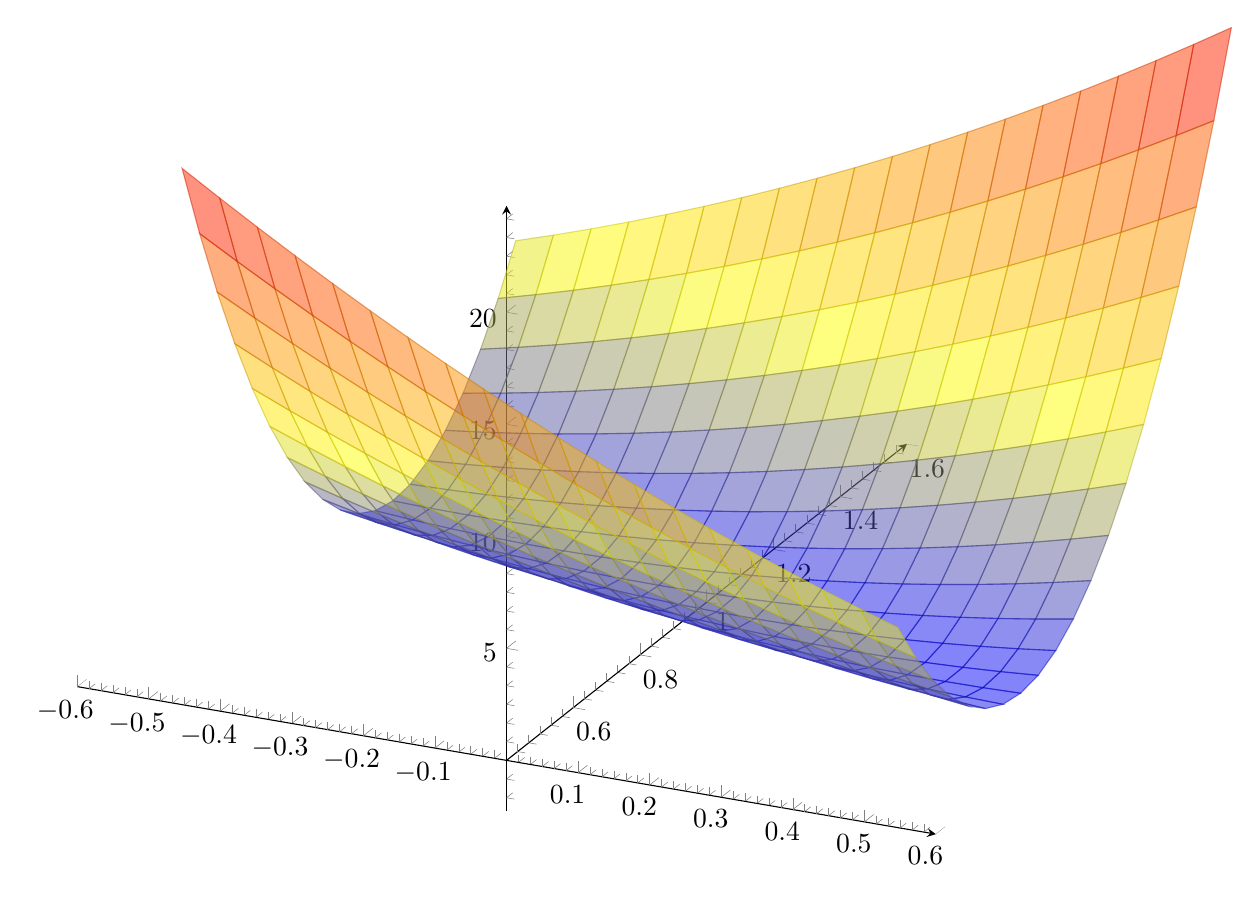
\begin{tikzpicture}[
	declare function = {
		N = 5;
		YSB = (1+4+9+16+25)/N;
		YXB = (1+4+9+16+25)/N;
		YB = (1+2+3+4+5)/N;
		XSB = (1+4+9+16+25)/N;
		XB = (1+2+3+4+5)/N;
		q(\x) = \x - 1;
		Z(\x,\y) = N*YSB -2*N*\y*YXB - 2*N*\x*YB + N*\y^2*XSB + 2*N*\x*\y*XB + N*\x^2;
	}
	]
	\begin{axis}
	[
	axis lines=center,
	enlargelimits,
	tick align=inside,
	domain=-0.5:0.5,
	domain y=0.5:1.5,
	samples=20,
	minor tick num=5,
	width=500
	]
	\addplot3 [surf, opacity=0.5] {Z(x,y)};	
	\end{axis}
	\end{tikzpicture}
	
	Now to find the line that minimizes the squared errors we can take the partial directives in relation to $w_0$ and $w_1$
	
	First partial derivative in relation of $w_0$
	\begin{align*}
		MSE_{line}&=\frac{d}{dw_0}[N\mean{y^2}-2Nw_1\mean{yx}-2Nw_0\mean{y}+Nw_1^2\mean{x^2}+2Nw_1w_0\mean{x}+Nw_0^2]\\
		&=\frac{d}{dw_0}[N\mean{y^2}]-\frac{d}{dw_0}[2Nw_1\mean{yx}]-\frac{d}{dw_0}[2Nw_0\mean{y}]+\frac{d}{dw_0}[Nw_1^2\mean{x^2}]+\frac{d}{dw_0}[2Nw_1w_0\mean{x}]+\frac{d}{dw_0}[Nw_0^2]\\
		&=-\frac{d}{dw_0}[2Nw_1\mean{yx}]-\frac{d}{dw_0}[2Nw_0\mean{y}]+\frac{d}{dw_0}[Nw_1^2\mean{x^2}]+\frac{d}{dw_0}[2Nw_1w_0\mean{x}]+\frac{d}{dw_0}[Nw_0^2]\\
		&=-\frac{d}{dw_0}[2Nw_0\mean{y}]+\frac{d}{dw_0}[Nw_1^2\mean{x^2}]+\frac{d}{dw_0}[2Nw_1w_0\mean{x}]+\frac{d}{dw_0}[Nw_0^2]\\
		&=-2N\mean{y}+\frac{d}{dw_0}[Nw_1^2\mean{x^2}]+\frac{d}{dw_0}[2Nw_1w_0\mean{x}]+\frac{d}{dw_0}[Nw_0^2]\\
		&=-2N\mean{y}+\frac{d}{dw_0}[2Nw_1w_0\mean{x}]+\frac{d}{dw_0}[Nw_0^2]\\
		&=-2N\mean{y}+2Nw_1\mean{x}+\frac{d}{dw_0}[Nw_0^2]\\
		&=-2N\mean{y}+2Nw_1\mean{x}+2Nw_0\\
	\end{align*}
	
	Now the derivative in relation to $w_1$
	\begin{align*}
		MSE_{line}&=\frac{d}{dw_1}[N\mean{y^2}-2Nw_1\mean{yx}-2Nw_0\mean{y}+Nw_1^2\mean{x^2}+2Nw_1w_0\mean{x}+Nw_0^2]\\
		&=\frac{d}{dw_1}[N\mean{y^2}]-\frac{d}{dw_1}[2Nw_1\mean{yx}]-\frac{d}{dw_1}[2Nw_0\mean{y}]+\frac{d}{dw_1}[Nw_1^2\mean{x^2}]+\frac{d}{dw_1}[2Nw_1w_0\mean{x}]+\frac{d}{dw_1}[Nw_0^2]\\
		&=-\frac{d}{dw_1}[2Nw_1\mean{yx}]-\frac{d}{dw_1}[2Nw_0\mean{y}]+\frac{d}{dw_1}[Nw_1^2\mean{x^2}]+\frac{d}{dw_1}[2Nw_1w_0\mean{x}]+\frac{d}{dw_1}[Nw_0^2]\\
		&=-2N\mean{yx}-\frac{d}{dw_1}[2Nw_0\mean{y}]+\frac{d}{dw_1}[Nw_1^2\mean{x^2}]+\frac{d}{dw_1}[2Nw_1w_0\mean{x}]+\frac{d}{dw_1}[Nw_0^2]\\
		&=-2N\mean{yx}+\frac{d}{dw_1}[Nw_1^2\mean{x^2}]+\frac{d}{dw_1}[2Nw_1w_0\mean{x}]+\frac{d}{dw_1}[Nw_0^2]\\
		&=-2N\mean{yx}+2Nw_1\mean{x^2}+\frac{d}{dw_1}[2Nw_1w_0\mean{x}]+\frac{d}{dw_1}[Nw_0^2]\\
		&=-2N\mean{yx}+2Nw_1\mean{x^2}+2Nw_0\mean{x}+\frac{d}{dw_1}[Nw_0^2]\\
		&=-2N\mean{yx}+2Nw_1\mean{x^2}+2Nw_0\mean{x}\\		
	\end{align*}
	
	Now we must solve the lienar system
	
	\begin{align*}
		\begin{cases}
			-2N\mean{y}+2Nw_1\mean{x}+2Nw_0=0\\
			-2N\mean{yx}+2Nw_1\mean{x^2}+2Nw_0\mean{x}=0
		\end{cases}\\
		&& \text{divide first 2N}\\
		\begin{cases}
			-\mean{y}+w_1\mean{x}+w_0=0\\
			-2N\mean{yx}+2Nw_1\mean{x^2}+2Nw_0\mean{x}=0
		\end{cases}\\
		&& \text{divide second 2N}\\
		\begin{cases}
			-\mean{y}+w_1\mean{x}+w_0=0\\
			-\mean{yx}+w_1\mean{x^2}+w_0\mean{x}=0
		\end{cases}\\
		\begin{cases}
			w_1\mean{x}+w_0=\mean{y}\\
			w_1\mean{x^2}+w_0\mean{x}=\mean{yx}
		\end{cases}\\
		\begin{cases}
			w_1\mean{x}+w_0=\mean{y}\\
			w_1\frac{\mean{x^2}}{\mean{x}}+w_0\frac{\mean{x}}{\mean{x}}=\frac{\mean{yx}}{\mean{x}}
		\end{cases}\\
		\begin{cases}
		w_1\mean{x}+w_0=\mean{y}\\
		w_1\frac{\mean{x^2}}{\mean{x}}+w_0=\frac{\mean{yx}}{\mean{x}}
		\end{cases}\\
	\end{align*}
	
	This means that the line that minimizes the squared error pass through the points
	\begin{align*}
		\big(\mean{x},\mean{y}\big)\\
		\big(\frac{\mean{x^2}}{\mean{x}},\frac{\mean{yx}}{\mean{x}}\big)\\
	\end{align*}
	
\end{document}